% Options for packages loaded elsewhere
\PassOptionsToPackage{unicode}{hyperref}
\PassOptionsToPackage{hyphens}{url}
%
\documentclass[
  11pt,
  a4paper,
]{article}
\usepackage{amsmath,amssymb}
\usepackage{lmodern}
\usepackage{iftex}
\ifPDFTeX
  \usepackage[T1]{fontenc}
  \usepackage[utf8]{inputenc}
  \usepackage{textcomp} % provide euro and other symbols
\else % if luatex or xetex
  \ifXeTeX
    \usepackage{zxjatype} 
    \usepackage[ipaex]{zxjafont}
    \setromanfont{Times New Roman}
  \fi
  \usepackage{unicode-math}
  \defaultfontfeatures{Scale=MatchLowercase}
  \defaultfontfeatures[\rmfamily]{Ligatures=TeX,Scale=1}
\fi
% Use upquote if available, for straight quotes in verbatim environments
\IfFileExists{upquote.sty}{\usepackage{upquote}}{}
\IfFileExists{microtype.sty}{% use microtype if available
  \usepackage[]{microtype}
  \UseMicrotypeSet[protrusion]{basicmath} % disable protrusion for tt fonts
}{}
\usepackage{xcolor}
\IfFileExists{xurl.sty}{\usepackage{xurl}}{} % add URL line breaks if available
\IfFileExists{bookmark.sty}{\usepackage{bookmark}}{\usepackage{hyperref}}
\hypersetup{
  pdftitle={Draft of Data and Estimation Result},
  hidelinks,
  pdfcreator={LaTeX via pandoc}}
\urlstyle{same} % disable monospaced font for URLs
\usepackage[left=3cm,right=3cm,top=3cm,bottom=3cm]{geometry}

\usepackage{setspace}
\renewcommand{\baselinestretch}{1.5}
\usepackage{float}

\usepackage{longtable,booktabs,array}
\usepackage{threeparttable, threeparttablex, multirow}
\usepackage{calc} % for calculating minipage widths
% Correct order of tables after \paragraph or \subparagraph
\usepackage{etoolbox}
\makeatletter
\patchcmd\longtable{\par}{\if@noskipsec\mbox{}\fi\par}{}{}
\makeatother
% Allow footnotes in longtable head/foot
\IfFileExists{footnotehyper.sty}{\usepackage{footnotehyper}}{\usepackage{footnote}}
\makesavenoteenv{longtable}
\usepackage{graphicx}
\makeatletter
\def\maxwidth{\ifdim\Gin@nat@width>\linewidth\linewidth\else\Gin@nat@width\fi}
\def\maxheight{\ifdim\Gin@nat@height>\textheight\textheight\else\Gin@nat@height\fi}
\makeatother
% Scale images if necessary, so that they will not overflow the page
% margins by default, and it is still possible to overwrite the defaults
% using explicit options in \includegraphics[width, height, ...]{}
\setkeys{Gin}{width=\maxwidth,height=\maxheight,keepaspectratio}
% Set default figure placement to htbp
\makeatletter
\def\fps@figure{htbp}
\makeatother
\setlength{\emergencystretch}{3em} % prevent overfull lines
\providecommand{\tightlist}{%
  \setlength{\itemsep}{0pt}\setlength{\parskip}{0pt}}
\setcounter{secnumdepth}{5}


\usepackage{booktabs}
\usepackage{siunitx}
\newcolumntype{d}{S[input-symbols = ()]}
\ifLuaTeX
  \usepackage{selnolig}  % disable illegal ligatures
\fi

\makeatletter
\def\@fnsymbol#1{\ensuremath{\ifcase#1\or \dagger\or \ddagger\or
   \mathsection\or \mathparagraph\or \|\or **\or \dagger\dagger
   \or \ddagger\ddagger \else\@ctrerr\fi}}
    \makeatother
\title{Draft of Data and Estimation Result  }
\author{
    Hiroki Kato
  \thanks{Graduate School of Economics, Osaka University, Japan. E-mail: vge008kh@stundent.econ.osaka-u.ac.jp  }
  \and
    Tsuyoshi Goto
  \thanks{Graduate School of Social Sciences, Chiba University, Japan. E-mail: t.goto@chiba-u.jp  }
  \and
    Youngrok Kim
  \thanks{Graduate School of Economics, Kobe University, Japan.  }
  \and
  }

\date{2022/02/17}


\begin{document}
\begin{spacing}{1}
  \maketitle
\end{spacing}

\hypertarget{national-survey-of-tax-and-benefit-nastab}{%
\subsection{National Survey of Tax and Benefit (NaSTaB)}\label{national-survey-of-tax-and-benefit-nastab}}

\begin{itemize}
\tightlist
\item
  2008年からKorea Institute of Taxation and Financeが実施
\item
  NaSTaBは家計の税負担や公的扶助などに関する年次パネルデータ
\item
  全国から5,634世帯を調査対象とする

  \begin{itemize}
  \tightlist
  \item
    5,634人の世帯主と15歳以上で経済活動をしている世帯員が調査に回答する
  \end{itemize}
\item
  我々の研究では(1)2013年から2018年かつ、(2)23歳以下の回答者を除いたデータを使用する

  \begin{itemize}
  \tightlist
  \item
    2012年と2013年の所得税率は変化していないが、2011年以前に所得税率の改正が何度か行われた (Table \ref{tab:TaxRate})
  \item
    2014年の制度改革に着目するために、2013年から2018年に限定する
  \item
    23歳以下の回答者は所得や資産を十分に持っていない可能性が高いので、データから除外する
  \end{itemize}
\end{itemize}

\hypertarget{descriptive-statistics}{%
\subsection{Descriptive Statistics}\label{descriptive-statistics}}

\begin{table}

\caption{\label{tab:SummaryCovariate}Descriptive Statistics}
\centering
\fontsize{6}{8}\selectfont
\begin{tabular}[t]{lcccccc}
\toprule
  & N & Mean & Std.Dev. & Min & Median & Max\\
\midrule
\addlinespace[0.3em]
\multicolumn{7}{l}{\textbf{Income and giving price}}\\
\hspace{1em}Annual taxable labor income (unit: 10,000KRW) & 36189 & \num{1747.26} & \num{2696.77} & \num{0.00} & \num{0.00} & \num{50000.00}\\
\hspace{1em}First giving relative price & 36198 & \num{0.86} & \num{0.04} & \num{0.62} & \num{0.85} & \num{0.94}\\
\addlinespace[0.3em]
\multicolumn{7}{l}{\textbf{Charitable giving}}\\
\hspace{1em}Annual chariatable giving (unit: 10,000KRW) & 36199 & \num{35.64} & \num{153.20} & \num{0.00} & \num{0.00} & \num{10000.00}\\
\hspace{1em}Dummary of donation > 0 & 36199 & \num{0.24} & \num{0.42} & \num{0.00} & \num{0.00} & \num{1.00}\\
\hspace{1em}Dummy of declaration of a tax relief & 36199 & \num{0.10} & \num{0.30} & \num{0.00} & \num{0.00} & \num{1.00}\\
\addlinespace[0.3em]
\multicolumn{7}{l}{\textbf{Individual Characteristics}}\\
\hspace{1em}Age & 36199 & \num{53.45} & \num{16.22} & \num{24.00} & \num{51.00} & \num{103.00}\\
\hspace{1em}Female dummy & 36199 & \num{0.43} & \num{0.50} & \num{0.00} & \num{0.00} & \num{1.00}\\
\hspace{1em}University graduate & 36198 & \num{0.42} & \num{0.49} & \num{0.00} & \num{0.00} & \num{1.00}\\
\hspace{1em}High school graduate dummy & 36198 & \num{0.31} & \num{0.46} & \num{0.00} & \num{0.00} & \num{1.00}\\
\hspace{1em}Junior high school graduate dummy & 36198 & \num{0.27} & \num{0.44} & \num{0.00} & \num{0.00} & \num{1.00}\\
\hspace{1em}Wage earner dummy & 27394 & \num{0.56} & \num{0.50} & \num{0.00} & \num{1.00} & \num{1.00}\\
\hspace{1em}\#.Tax accountant / population & 36199 & \num{1.04} & \num{0.51} & \num{0.32} & \num{0.92} & \num{2.24}\\
\bottomrule
\end{tabular}
\end{table}

\hypertarget{ux53f3ux6b6aux66f2ux306eux6240ux5f97ux5206ux5e03ux3068ux5bc4ux4ed8ux4fa1ux683cux306eux5909ux52d5}{%
\subsection{右歪曲の所得分布と寄付価格の変動}\label{ux53f3ux6b6aux66f2ux306eux6240ux5f97ux5206ux5e03ux3068ux5bc4ux4ed8ux4fa1ux683cux306eux5909ux52d5}}

\begin{figure}[t]

{\centering 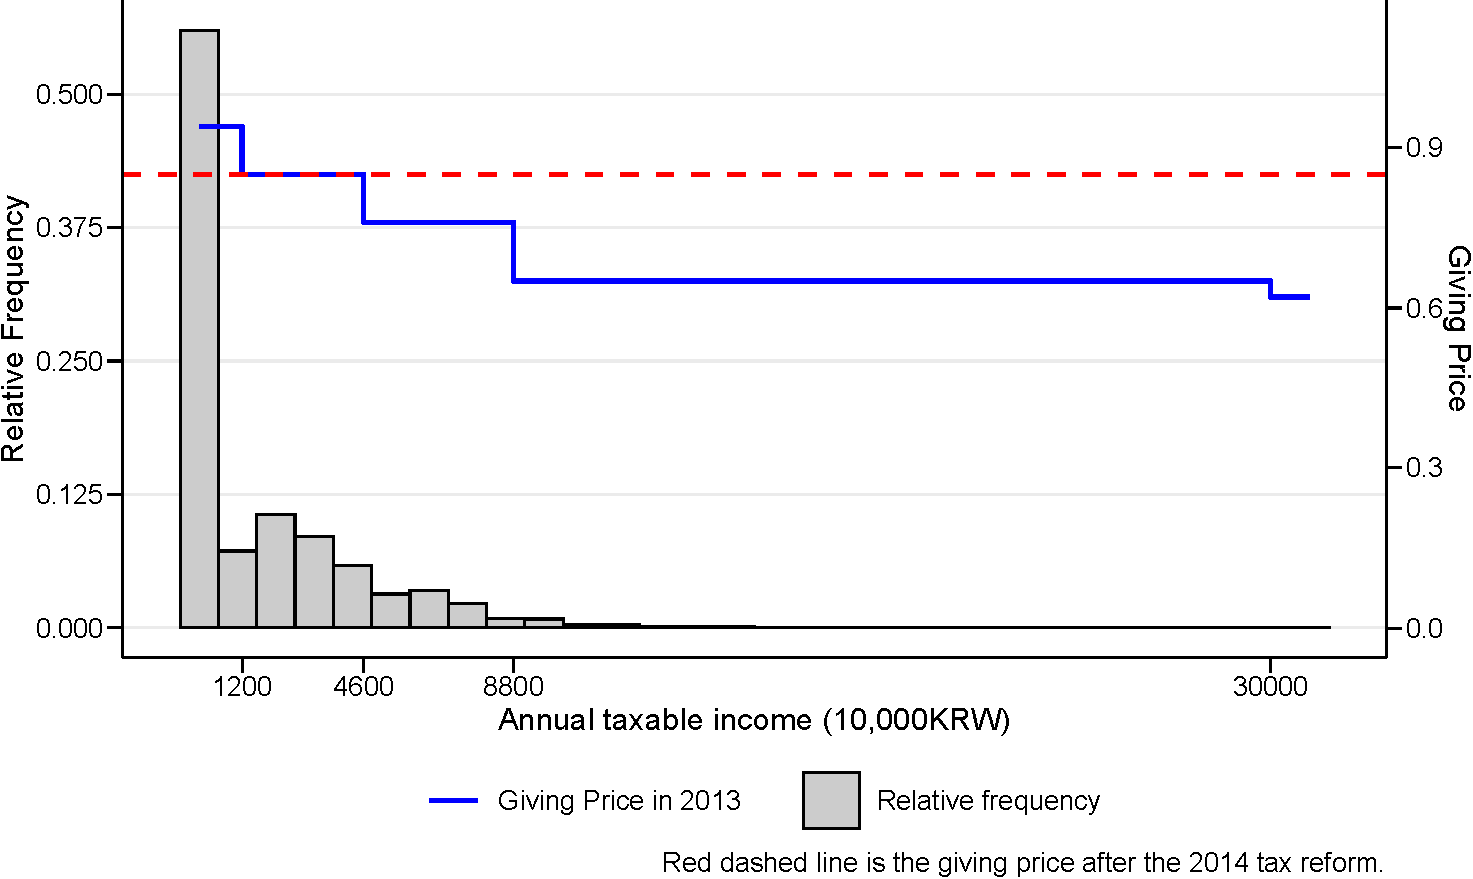
\includegraphics{C:/Users/vge00/Desktop/NASTAB/paper/draft_files/figure-latex/SummaryPrice-1} 

}

\caption{Income Distribution in 2013 and Relative Giving Price. Notes: The left and right axis measure the relative frequency of respondents (grey bars) and the relative giving price (solid step line and dashed line), respectively. A solid step line and a dashed horizontal line represents the giving price in 2013 and 2014, respectively.}\label{fig:SummaryPrice}
\end{figure}

\hypertarget{ux5e74ux7a0eux5236ux6539ux9769ux76f4ux5f8cux5bc4ux4ed8ux8005ux6bd4ux7387ux304cux6e1bux5c11}{%
\subsection{2014年税制改革直後、寄付者比率が減少}\label{ux5e74ux7a0eux5236ux6539ux9769ux76f4ux5f8cux5bc4ux4ed8ux8005ux6bd4ux7387ux304cux6e1bux5c11}}

\begin{figure}[t]

{\centering 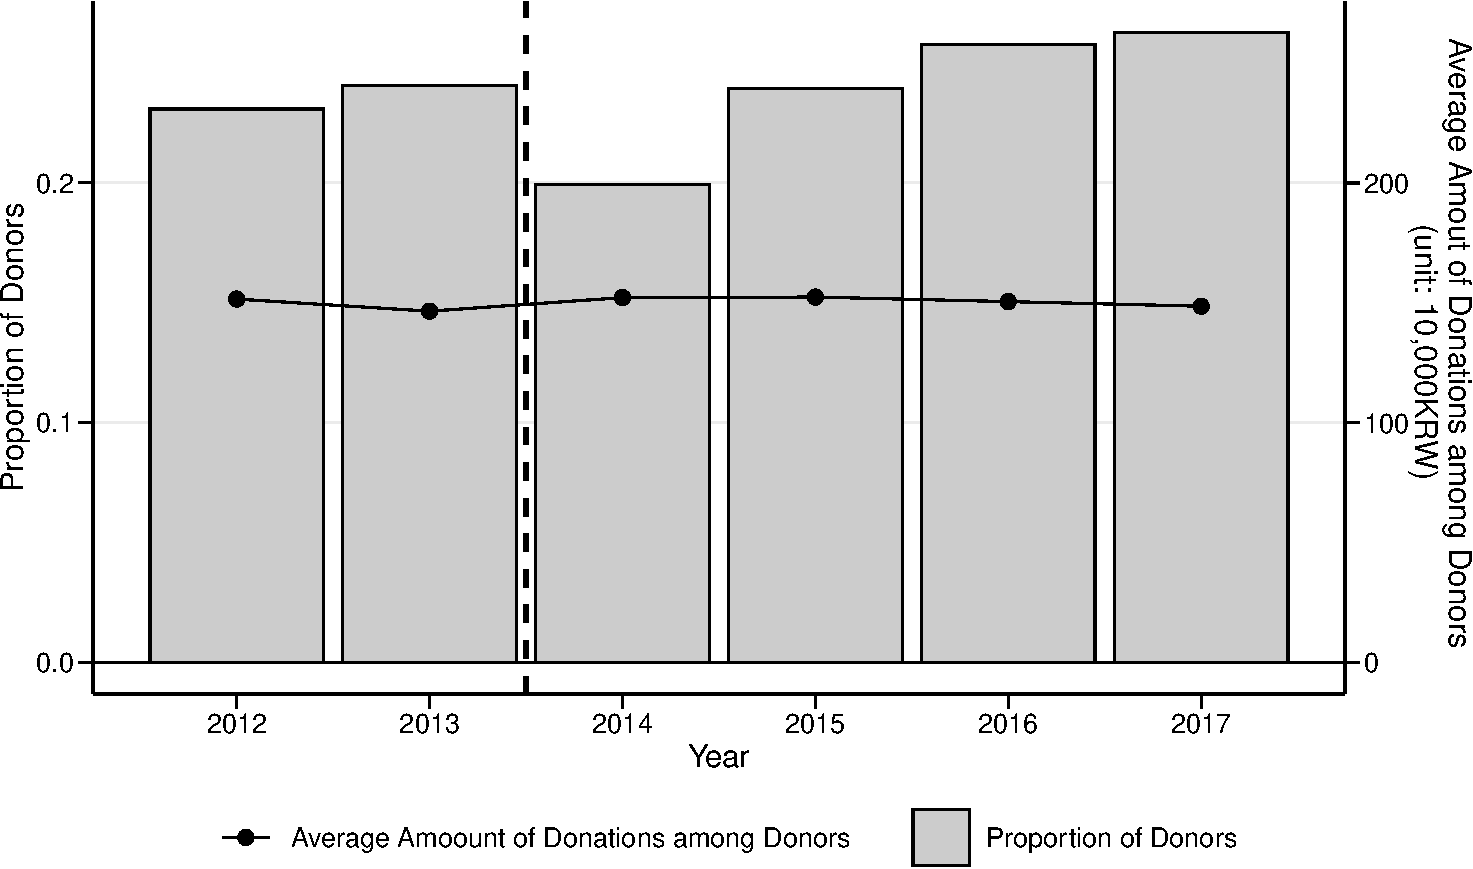
\includegraphics{C:/Users/vge00/Desktop/NASTAB/paper/draft_files/figure-latex/SummaryGiving-1} 

}

\caption{Proportion of Donors and Average Donations among Donors. Notes: The left and right axises measure prooortion of donors (grey bars) and the average amount of donations among donors (solid line), respectively.}\label{fig:SummaryGiving}
\end{figure}

\hypertarget{ux7a0eux30a4ux30f3ux30bbux30f3ux30c6ux30a3ux30d6ux306fux5bc4ux4ed8ux984dux3092ux5897ux3084ux3057ux305f}{%
\subsection{税インセンティブは寄付額を増やした}\label{ux7a0eux30a4ux30f3ux30bbux30f3ux30c6ux30a3ux30d6ux306fux5bc4ux4ed8ux984dux3092ux5897ux3084ux3057ux305f}}

\begin{figure}[t]

{\centering 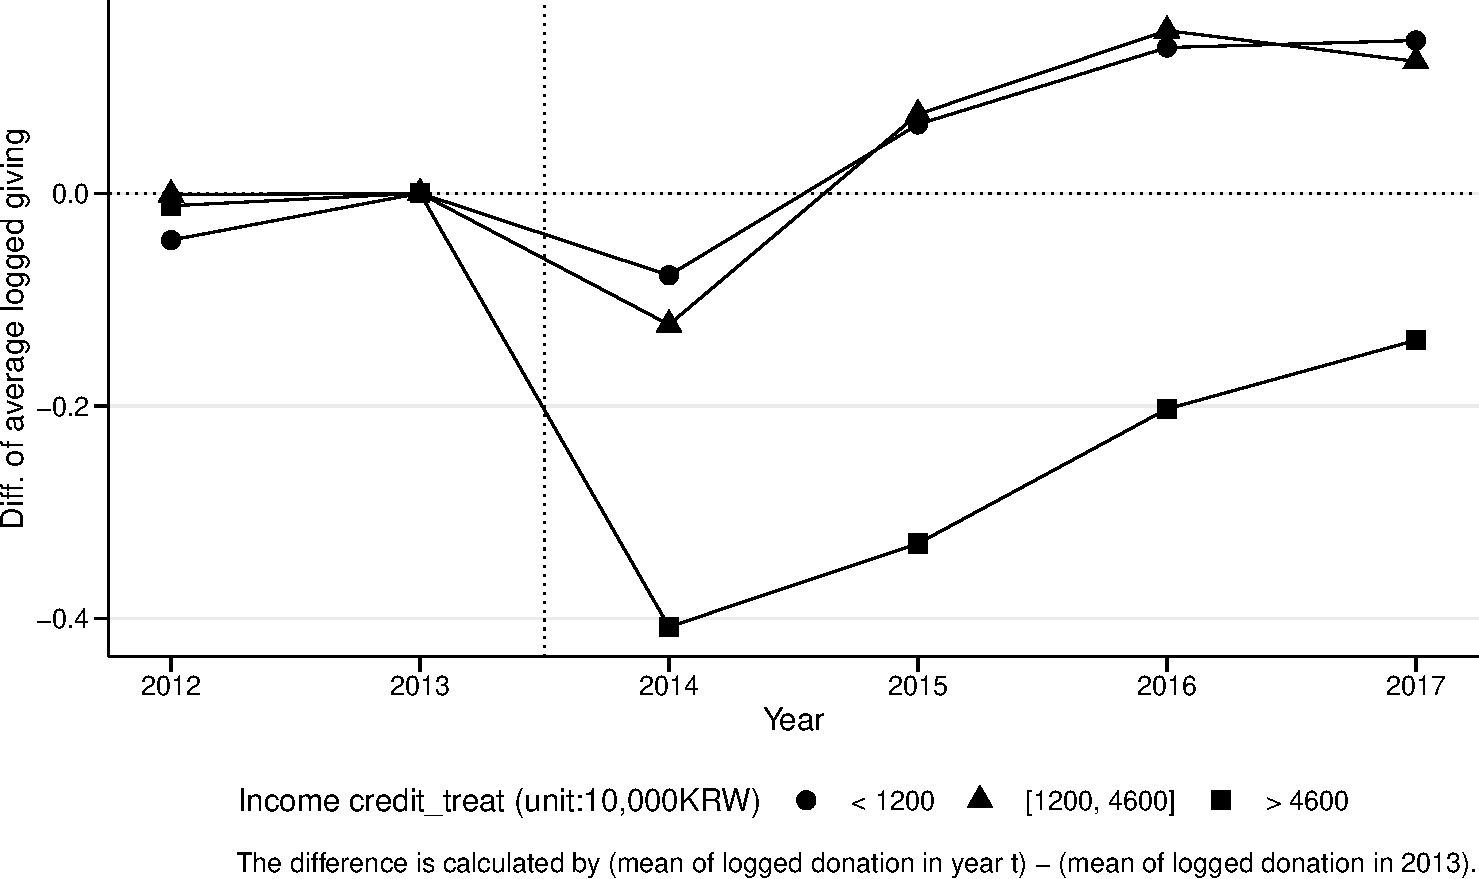
\includegraphics{C:/Users/vge00/Desktop/NASTAB/paper/draft_files/figure-latex/SummaryGivingOverall-1} 

}

\caption{Average Logged Giving by Three Income Groups. Notes: We created three income groups, with the relative price of giving rising (circle), unchanged (triangle), and falling (square) between 2013 and 2014. The group averages are normalized to be zero in 2013.}\label{fig:SummaryGivingOverall}
\end{figure}

\hypertarget{ux5bc4ux4ed8ux8005ux306bux9650ux5b9aux3059ux308bux3068ux5bc4ux4ed8ux984dux306bux5bfeux3059ux308bux4fa1ux683cux52b9ux679cux306fux306fux3063ux304dux308aux3068ux3057ux306aux3044}{%
\subsection{寄付者に限定すると、寄付額に対する価格効果ははっきりとしない}\label{ux5bc4ux4ed8ux8005ux306bux9650ux5b9aux3059ux308bux3068ux5bc4ux4ed8ux984dux306bux5bfeux3059ux308bux4fa1ux683cux52b9ux679cux306fux306fux3063ux304dux308aux3068ux3057ux306aux3044}}

\begin{figure}[t]

{\centering 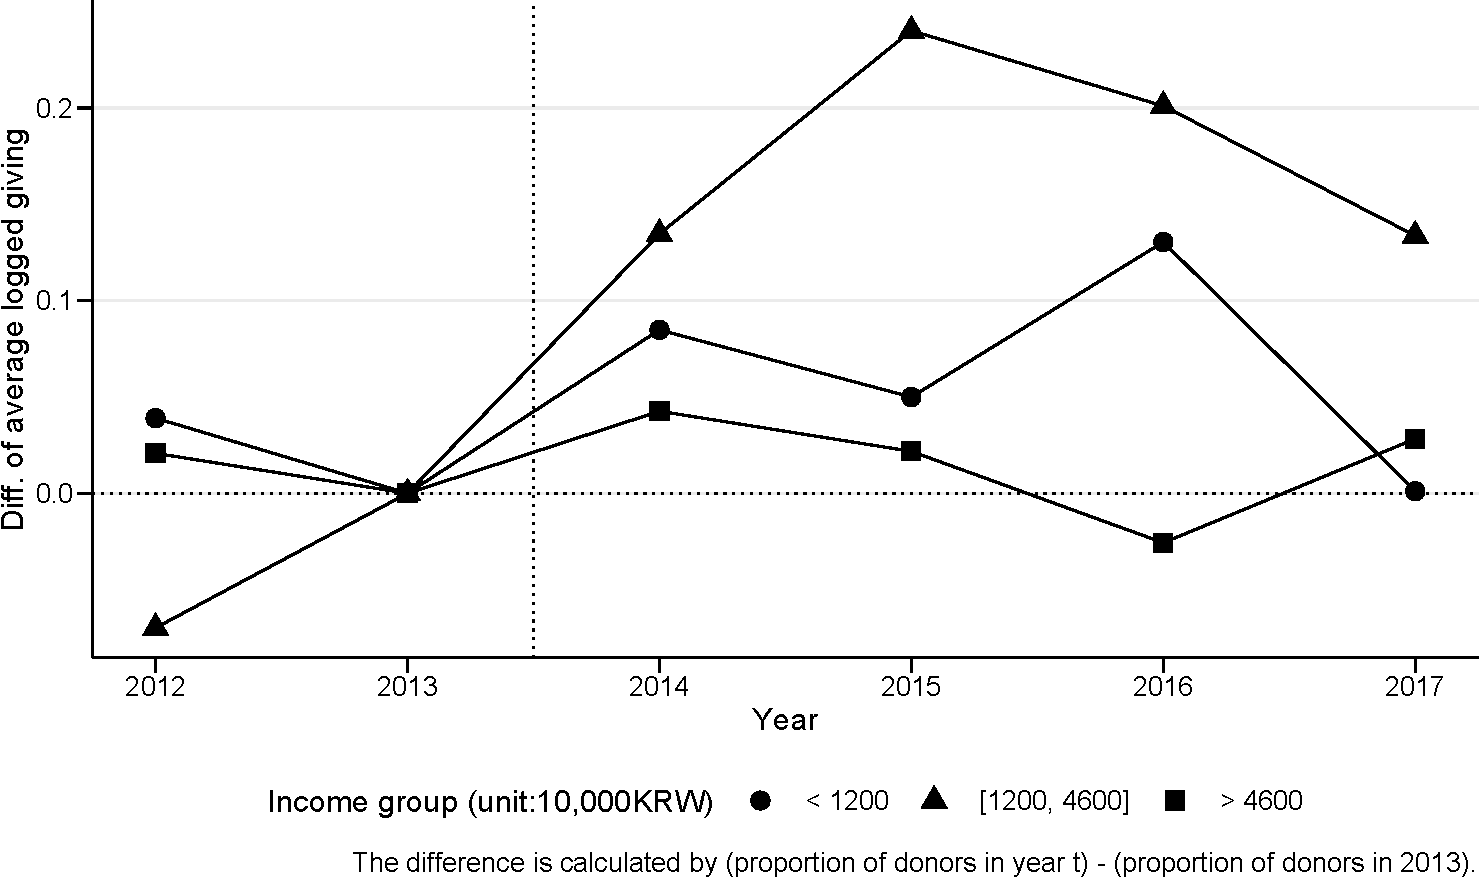
\includegraphics{C:/Users/vge00/Desktop/NASTAB/paper/draft_files/figure-latex/SummaryGivingIntensive-1} 

}

\caption{Average Logged Giving by Three Income Groups Conditional on Donors. Notes: We created three income groups, with the relative price of giving rising (circle), unchanged (triangle), and falling (square) between 2013 and 2014. The group averages are normalized to be zero in 2013.}\label{fig:SummaryGivingIntensive}
\end{figure}

\hypertarget{ux7a0eux30a4ux30f3ux30bbux30f3ux30c6ux30a3ux30d6ux306fux5bc4ux4ed8ux8005ux3092ux5897ux3084ux3057ux305f}{%
\subsection{税インセンティブは寄付者を増やした}\label{ux7a0eux30a4ux30f3ux30bbux30f3ux30c6ux30a3ux30d6ux306fux5bc4ux4ed8ux8005ux3092ux5897ux3084ux3057ux305f}}

\begin{figure}[t]

{\centering 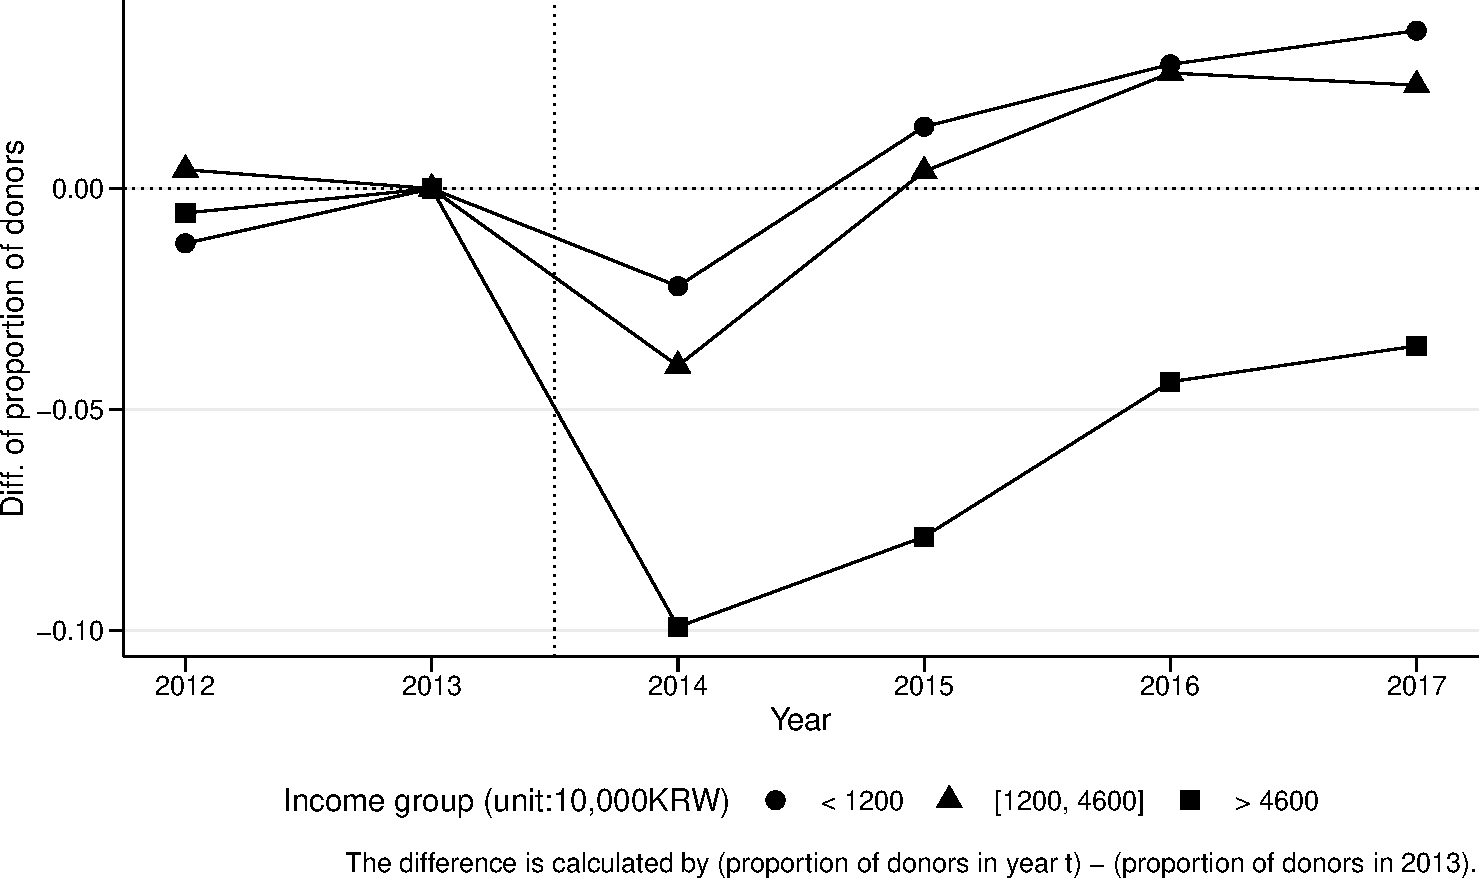
\includegraphics{C:/Users/vge00/Desktop/NASTAB/paper/draft_files/figure-latex/SummaryGivingExtensive-1} 

}

\caption{Proportion of Donors by Three Income Groups. Notes: We created three income groups, with the relative price of giving rising (circle), unchanged (triangle), and falling (square) between 2013 and 2014. The group averages are normalized to be zero in 2013.}\label{fig:SummaryGivingExtensive}
\end{figure}

\hypertarget{ux5236ux5ea6ux6539ux9769ux306bux95a2ux308fux3089ux305aux7d66ux4e0eux6240ux5f97ux8005ux306fux5bc4ux4ed8ux7533ux544aux3092ux3057ux3084ux3059ux3044}{%
\subsection{制度改革に関わらず、給与所得者は寄付申告をしやすい}\label{ux5236ux5ea6ux6539ux9769ux306bux95a2ux308fux3089ux305aux7d66ux4e0eux6240ux5f97ux8005ux306fux5bc4ux4ed8ux7533ux544aux3092ux3057ux3084ux3059ux3044}}

\begin{figure}[t]

{\centering 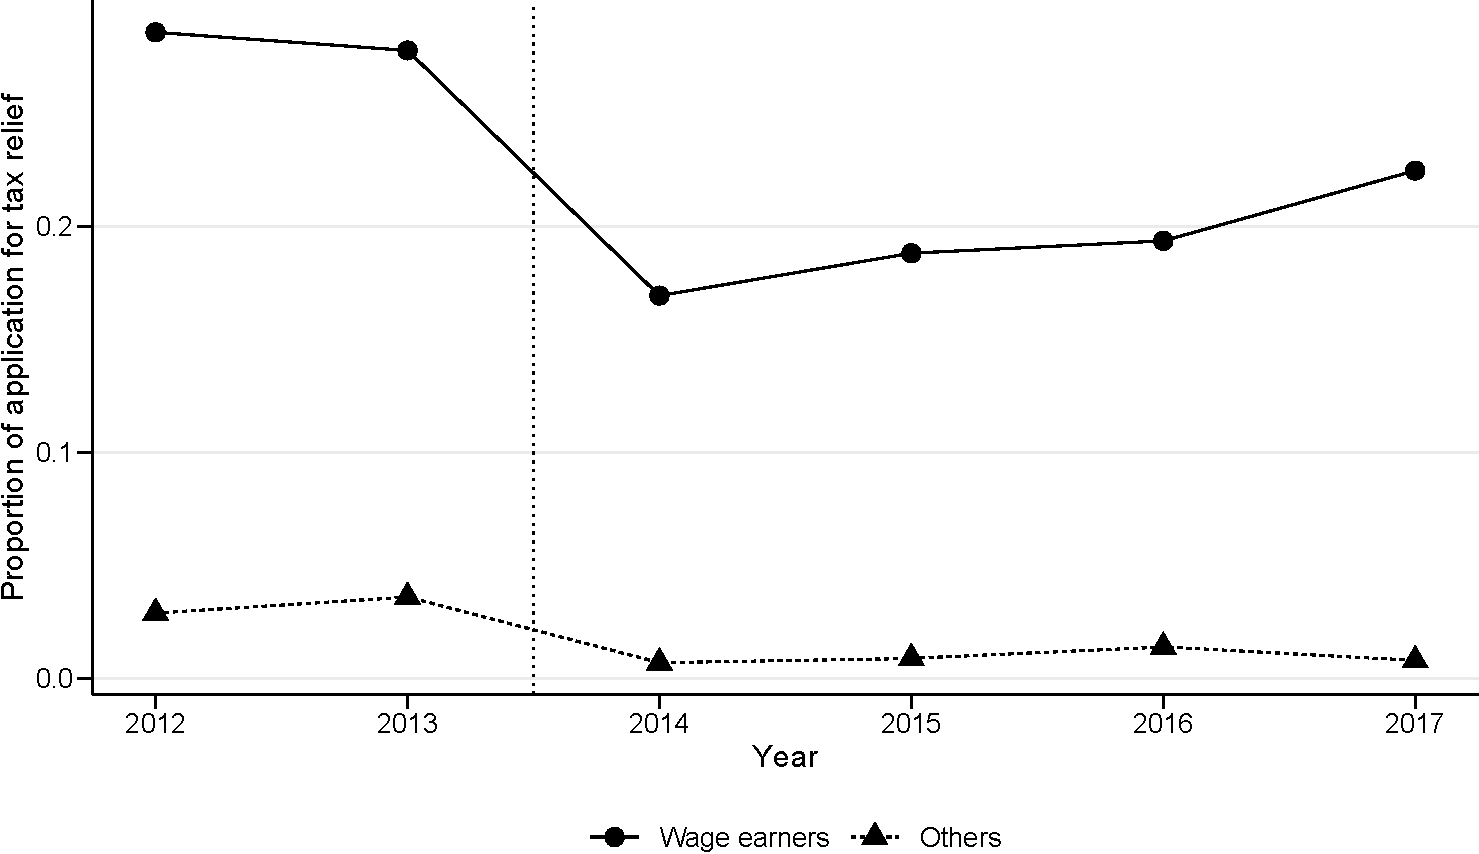
\includegraphics{C:/Users/vge00/Desktop/NASTAB/paper/draft_files/figure-latex/SummaryReliefbyEarner-1} 

}

\caption{Share of Tax Relief by Wage Earners. Notes: A solid line is the share of applying for tax relief among wage eaners. A dashed line is the share of applying for tax relief other than wage earners.}\label{fig:SummaryReliefbyEarner}
\end{figure}

\hypertarget{ux7a2eux985eux306eux5bc4ux4ed8ux306eux4fa1ux683cux5f3eux529bux6027}{%
\subsection{2種類の寄付の価格弾力性}\label{ux7a2eux985eux306eux5bc4ux4ed8ux306eux4fa1ux683cux5f3eux529bux6027}}

(\textbf{Scharf2020?}) に従い、2種類の価格弾力性を推定する

\begin{enumerate}
\def\labelenumi{\arabic{enumi}.}
\tightlist
\item
  Intensive-margin tax-price elasticity: 1\%の価格上昇で寄付者の寄付額が何\%増えるか?
\item
  Extensive-margin tax-price elasticity: 1\%の価格上昇で寄付確率が何\%増えるか?
\end{enumerate}

\hypertarget{intensive-margin-tax-price-elasticityux306eux63a8ux5b9aux65b9ux6cd5}{%
\subsection{Intensive-Margin Tax-Price Elasticityの推定方法}\label{intensive-margin-tax-price-elasticityux306eux63a8ux5b9aux65b9ux6cd5}}

\begin{align}
  \ln g_{it} = \theta_i + \gamma (R_{it} \times \ln (1 - s_{it}))
  + \beta X_{it} + \lambda_t + u_{it}, \label{eq:intensive}
\end{align}

\begin{itemize}
\tightlist
\item
  \(X_{it}\)は課税前所得(\(y_{it}\))を含んだ共変量ベクトル
\item
  \(\theta_i\)は個人固定効果、\(\lambda_t\)は時間固定効果
\item
  \(u_{it}\)はidiosyncratic error
\item
  関心のあるパラメータは\(\gamma\)で、intensive-margin tax-price elasticityを示す
\end{itemize}

\hypertarget{extensive-margin-tax-price-elasticityux306eux63a8ux5b9aux65b9ux6cd5}{%
\subsection{Extensive-Margin Tax-Price Elasticityの推定方法}\label{extensive-margin-tax-price-elasticityux306eux63a8ux5b9aux65b9ux6cd5}}

\begin{align}
  D_{it} = \theta_i + \delta (R_{it} \times \ln (1 - s_{it}))
  + \beta X_{it} + \lambda_t + u_{it}, \label{eq:extensive}
\end{align}

\begin{itemize}
\tightlist
\item
  \(D_{it}\)は正の寄付額(\(g_{it} > 0\))が観測されたら1を取るダミー変数
\item
  関心のあるパラメータは\(\delta\)

  \begin{itemize}
  \tightlist
  \item
    二値のアウトカム変数なので、\(\delta\)は直接、価格弾力性として解釈できない
  \item
    Extensive-Margin Tax-Price Elasticityは\(\hat{\delta} / \bar{D}\)で得られる(\(\bar{D}\)は\(D_{it}\)の標本平均)
  \end{itemize}
\end{itemize}

\hypertarget{ux5bc4ux4ed8ux306eux76f8ux5bfeux4fa1ux683cux306eux5185ux751fux6027}{%
\subsection{寄付の相対価格の内生性}\label{ux5bc4ux4ed8ux306eux76f8ux5bfeux4fa1ux683cux306eux5185ux751fux6027}}

\begin{align}
  1 - s_{it} =
  \begin{cases}
    1 - T'_t(y_{it} - g_{it})  \quad\text{if}\quad t < 2014  \\
    1 - m \quad\text{if}\quad t \ge 2014
  \end{cases},
\end{align}

\begin{itemize}
\tightlist
\item
  \(T'_t(\cdot)\)は\(t\)年の限界所得税率、\(m\)は税額控除率(\(m = 0.15\))
\item
  所得控除のとき、寄付価格は寄付額(\(g_{it}\))に依存する
\item
  この価格は\emph{Last}-unit priceと呼ばれる
\end{itemize}

過去の研究にならい、本研究は以下の\emph{first}-unit priceを\emph{last}-unit priceの代わり(もしくはその操作変数)として用いる

\begin{align}
  1 - s^f_{it} =
  \begin{cases}
    1 - T'_t(y_{it} - 0)  \quad\text{if}\quad t < 2014  \\
    1 - m \quad\text{if}\quad t \ge 2014
  \end{cases},
\end{align}

\hypertarget{ux5bc4ux4ed8ux7533ux544aux306eux5185ux751fux6027}{%
\subsection{寄付申告の内生性}\label{ux5bc4ux4ed8ux7533ux544aux306eux5185ux751fux6027}}

給与所得者ダミーをIVとして用いる

\begin{itemize}
\tightlist
\item
  所得や業種をコントロールすれば、給与所得者であるかどうかは直接寄付額に影響しない
\item
  給与所得者のほうが非給与所得者より寄付申告コストが安いと考えられる
\end{itemize}

(\textbf{Wooldridge2010a?}) より、以下の二つの方法で推定する

\begin{enumerate}
\def\labelenumi{\arabic{enumi}.}
\tightlist
\item
  給与所得者ダミー(\(Z_{it}\))とfirst-unit priceの交差項を\(R_{it} \times \ln (1 - s^f_{it})\)の操作変数として用いる
\item
  寄付申告の傾向スコア\(P_{it}\)とfirst-unit priceの交差項を操作変数として用いる

  \begin{itemize}
  \tightlist
  \item
    傾向スコア\(P_{it}\)は\(R_{it} = 1[\alpha_0 + \alpha_1 Z_{it} + \alpha_2 \ln(1 - s^f_{it}) + \alpha_3 X_{it} + u_{it0} > 0]\)をプロビット推定し、その予測確率で得る
  \item
    プロビット推定は係数が時間に対して一定と仮定したPooledモデルと係数が時間に対して異なると仮定したSeparatedモデルで推定
  \end{itemize}
\end{enumerate}

\hypertarget{ux7d50ux679c-intensive-margin-tax-price-elasticity}{%
\subsection{結果: Intensive-Margin Tax-Price Elasticity}\label{ux7d50ux679c-intensive-margin-tax-price-elasticity}}

\begin{table}

\caption{\label{tab:MainIntensive}Intensive-Margin Tax-Price Elasticity}
\centering
\fontsize{7}{9}\selectfont
\begin{threeparttable}
\begin{tabular}[t]{lcccccc}
\toprule
\multicolumn{1}{c}{ } & \multicolumn{3}{c}{FE} & \multicolumn{3}{c}{FE-2SLS} \\
\cmidrule(l{3pt}r{3pt}){2-4} \cmidrule(l{3pt}r{3pt}){5-7}
  & (1) & (2) & (3) & (4) & (5) & (6)\\
\midrule
Applying tax relief x log(first price) & \num{-0.748}*** &  &  & \num{-1.400}*** & \num{-1.437}*** & \num{-1.540}***\\
 & (\num{0.225}) &  &  & (\num{0.411}) & (\num{0.363}) & (\num{0.375})\\
PS of applying tax relief x log(first price) &  & \num{-1.544}*** & \num{-1.515}*** &  &  & \\
 &  & (\num{0.388}) & (\num{0.367}) &  &  & \\
\midrule
First-stage: Instrument &  &  &  & 0.638 & 1.075 & 0.984\\
 &  &  &  & {}[468.1] & {}[534.6] & {}[662.2]\\
Num.Obs. & \num{7004} & \num{6975} & \num{6975} & \num{6975} & \num{6975} & \num{6975}\\
Instrument &  &  &  & WE x Price & PS x Price & PS x Price\\
Method of PS &  & Pool & Separate &  & Pool & Separate\\
\bottomrule
\multicolumn{7}{l}{\rule{0pt}{1em}* p $<$ 0.1, ** p $<$ 0.05, *** p $<$ 0.01}\\
\end{tabular}
\begin{tablenotes}
\item Notes: $^{*}$ $p < 0.1$, $^{**}$ $p < 0.05$, $^{***}$ $p < 0.01$. Standard errors are clustered at individual level. A square bracket is wald statistics of instrument.
\end{tablenotes}
\end{threeparttable}
\end{table}

\hypertarget{ux7d50ux679c-extensive-margin-tax-price-elasticity}{%
\subsection{結果: Extensive-Margin Tax-Price Elasticity}\label{ux7d50ux679c-extensive-margin-tax-price-elasticity}}

\begin{table}

\caption{\label{tab:MainExtensive}Extensive-Margin Tax-Price Elasticity}
\centering
\fontsize{7}{9}\selectfont
\begin{threeparttable}
\begin{tabular}[t]{lcccccc}
\toprule
\multicolumn{1}{c}{ } & \multicolumn{3}{c}{FE} & \multicolumn{3}{c}{FE-2SLS} \\
\cmidrule(l{3pt}r{3pt}){2-4} \cmidrule(l{3pt}r{3pt}){5-7}
  & (1) & (2) & (3) & (4) & (5) & (6)\\
\midrule
Applying tax relief x log(first price) & \num{-2.800}*** &  &  & \num{-0.464}*** & \num{-0.563}*** & \num{-0.738}***\\
 & (\num{0.074}) &  &  & (\num{0.176}) & (\num{0.120}) & (\num{0.116})\\
PS of applying tax relief x log(first price) &  & \num{-0.452}*** & \num{-0.566}*** &  &  & \\
 &  & (\num{0.107}) & (\num{0.101}) &  &  & \\
\midrule
Implied price elasticity & -10.799*** & -1.741*** & -2.181*** & -1.788*** & -2.169*** & -2.841***\\
 & (0.287) & (0.411) & (0.388) & (0.678) & (0.463) & (0.448)\\
First-stage: Instrument &  &  &  & 0.289 & 0.803 & 0.768\\
 &  &  &  & {}[276.6] & {}[311.7] & {}[361.9]\\
Num.Obs. & \num{27017} & \num{26863} & \num{26863} & \num{26863} & \num{26863} & \num{26863}\\
Instrument &  &  &  & WE x Price & PS x Price & PS x Price\\
Method of PS &  & Pool & Separate &  & Pool & Separate\\
\bottomrule
\multicolumn{7}{l}{\rule{0pt}{1em}* p $<$ 0.1, ** p $<$ 0.05, *** p $<$ 0.01}\\
\end{tabular}
\begin{tablenotes}
\item Notes: $^{*}$ $p < 0.1$, $^{**}$ $p < 0.05$, $^{***}$ $p < 0.01$. Standard errors are clustered at individual level. A square bracket is wald statistics of instrument.
\end{tablenotes}
\end{threeparttable}
\end{table}

\hypertarget{ux30edux30d0ux30b9ux30c8ux30cdux30b9ux30c1ux30a7ux30c3ux30af}{%
\subsection{ロバストネスチェック}\label{ux30edux30d0ux30b9ux30c8ux30cdux30b9ux30c1ux30a7ux30c3ux30af}}

\begin{enumerate}
\def\labelenumi{\arabic{enumi}.}
\tightlist
\item
  2013-2014年データを除外 (Table \ref{tab:WoAnnoucementIntensive} and \ref{tab:WoAnnouncementExtensive})

  \begin{itemize}
  \tightlist
  \item
    税制改革のアナウンスメント効果を排除
  \end{itemize}
\item
  First-unit priceではなく、Last-unit priceで弾力性を推定 (Table \ref{tab:LastIntensive} and \ref{tab:LastExtensive})
\item
  給与所得者ダミーと寄付価格の交差項ではなく、first-unit priceを操作変数にする (Table \ref{tab:MainElasticity}-\ref{tab:WoAnnoucementElasticity})
\item
  寄付申告者に限定し、所得控除制度による内生性(e.g.~所得の変動)を考慮した分析を実施 (Table \ref{tab:R1Elasticity} and \ref{tab:KdiffElasticity})

  \begin{itemize}
  \tightlist
  \item
    階差モデルやリードラグ変数の使用 (Gruber and Saez, 2002; Randolph, 1995; \textbf{Scharf2020?})
  \end{itemize}
\end{enumerate}

ほとんどの分析で、intensive-margin tax-price elasticityは-1.5から-2の間に入り、
extensive-margin tax-price elasticityは-1.7から-5の間に入る

\hypertarget{ux97d3ux56fdux3067ux306eux5bc4ux4ed8ux306eux4fa1ux683cux5f3eux529bux6027ux306fux5148ux884cux7814ux7a76ux3088ux308aux5f3eux529bux7684}{%
\subsection{韓国での寄付の価格弾力性は先行研究より弾力的}\label{ux97d3ux56fdux3067ux306eux5bc4ux4ed8ux306eux4fa1ux683cux5f3eux529bux6027ux306fux5148ux884cux7814ux7a76ux3088ux308aux5f3eux529bux7684}}

\begin{itemize}
\tightlist
\item
  申告の自己選択を無視すると、Intensive-margin tax-price elasticityは過小推定

  \begin{itemize}
  \tightlist
  \item
    寄付者の寄付額を決める観察できない要素と申告が正の相関をしている
  \item
    そのような要素を寄付額を高めるならば、節税による便益が高くなるので、申告しやすくなる
  \end{itemize}
\item
  申告の自己選択を無視すると、Extensive-margin tax-price elasticityは過大推定

  \begin{itemize}
  \tightlist
  \item
    寄付価格が申告と寄付するかどうかの意思決定の両方に同じ方向の影響を与え、負の相関をより強くした可能性がある
  \end{itemize}
\end{itemize}

\hypertarget{conventional-method-to-estimate-tax-price-elasticity}{%
\subsection{Conventional Method to Estimate Tax-Price Elasticity}\label{conventional-method-to-estimate-tax-price-elasticity}}

\begin{table}

\caption{\label{tab:MainElasticity}Estimation of Last-Unit Price Elasticities}
\centering
\fontsize{7}{9}\selectfont
\begin{threeparttable}
\begin{tabular}[t]{lcccc}
\toprule
\multicolumn{1}{c}{ } & \multicolumn{2}{c}{Intensive margin} & \multicolumn{2}{c}{Extensive margin} \\
\cmidrule(l{3pt}r{3pt}){2-3} \cmidrule(l{3pt}r{3pt}){4-5}
\multicolumn{1}{c}{ } & \multicolumn{1}{c}{FE} & \multicolumn{1}{c}{FE-2SLS} & \multicolumn{1}{c}{FE} & \multicolumn{1}{c}{FE-2SLS} \\
\cmidrule(l{3pt}r{3pt}){2-2} \cmidrule(l{3pt}r{3pt}){3-3} \cmidrule(l{3pt}r{3pt}){4-4} \cmidrule(l{3pt}r{3pt}){5-5}
  & (1) & (2) & (3) & (4)\\
\midrule
log(last price) & \num{-0.634}*** & \num{-1.907}*** & \num{-2.945}*** & \num{-1.570}***\\
 & (\num{0.231}) & (\num{0.451}) & (\num{0.071}) & (\num{0.127})\\
\midrule
Implied price elasticity &  &  & -11.684*** & -6.227***\\
 &  &  & (0.281) & (0.502)\\
First-stage: log(first price) &  & 0.726 &  & 0.353\\
 &  & {}[442.4] &  & {}[407.8]\\
Num.Obs. & \num{7234} & \num{7234} & \num{28696} & \num{28696}\\
\bottomrule
\multicolumn{5}{l}{\rule{0pt}{1em}* p $<$ 0.1, ** p $<$ 0.05, *** p $<$ 0.01}\\
\end{tabular}
\begin{tablenotes}
\item Notes: $^{*}$ $p < 0.1$, $^{**}$ $p < 0.05$, $^{***}$ $p < 0.01$. Standard errors are clustered at individual level. A square bracket is wald statistics of instrument.
\end{tablenotes}
\end{threeparttable}
\end{table}

\hypertarget{conventional-method-to-estimate-tax-price-elasticity-2}{%
\subsection{Conventional Method to Estimate Tax-Price Elasticity (2)}\label{conventional-method-to-estimate-tax-price-elasticity-2}}

\begin{table}

\caption{\label{tab:WoAnnoucementElasticity}Estimation of Last-Unit Price Elasticities Excluding 2013 and 2014 data}
\centering
\fontsize{7}{9}\selectfont
\begin{threeparttable}
\begin{tabular}[t]{lcccc}
\toprule
\multicolumn{1}{c}{ } & \multicolumn{2}{c}{Intensive margin} & \multicolumn{2}{c}{Extensive margin} \\
\cmidrule(l{3pt}r{3pt}){2-3} \cmidrule(l{3pt}r{3pt}){4-5}
\multicolumn{1}{c}{ } & \multicolumn{1}{c}{FE} & \multicolumn{1}{c}{FE-2SLS} & \multicolumn{1}{c}{FE} & \multicolumn{1}{c}{FE-2SLS} \\
\cmidrule(l{3pt}r{3pt}){2-2} \cmidrule(l{3pt}r{3pt}){3-3} \cmidrule(l{3pt}r{3pt}){4-4} \cmidrule(l{3pt}r{3pt}){5-5}
  & (1) & (2) & (3) & (4)\\
\midrule
log(last price) & \num{-0.679}** & \num{-2.088}*** & \num{-3.097}*** & \num{-1.560}***\\
 & (\num{0.333}) & (\num{0.600}) & (\num{0.086}) & (\num{0.170})\\
\midrule
Implied price elasticity &  &  & -11.574*** & -5.830***\\
 &  &  & (0.320) & (0.634)\\
First-stage: log(first price) &  & 0.796 &  & 0.363\\
 &  & {}[270.6] &  & {}[244.3]\\
Num.Obs. & \num{5405} & \num{5405} & \num{20198} & \num{20198}\\
\bottomrule
\multicolumn{5}{l}{\rule{0pt}{1em}* p $<$ 0.1, ** p $<$ 0.05, *** p $<$ 0.01}\\
\end{tabular}
\begin{tablenotes}
\item Notes: $^{*}$ $p < 0.1$, $^{**}$ $p < 0.05$, $^{***}$ $p < 0.01$. Standard errors are clustered at individual level. A square bracket is wald statistics of instrument.
\end{tablenotes}
\end{threeparttable}
\end{table}

\hypertarget{estimating-price-elasticity-using-compliers}{%
\subsection{Estimating Price Elasticity Using Compliers}\label{estimating-price-elasticity-using-compliers}}

\begin{table}

\caption{\label{tab:R1Elasticity}Estimating Intensive-Margin Price Elasticities for Those Who Applied for Tax Relief}
\centering
\fontsize{5}{7}\selectfont
\begin{threeparttable}
\begin{tabular}[t]{lcccc}
\toprule
  & (1) & (2) & (3) & (4)\\
\midrule
log(first price) & \num{-1.203}*** & \num{-0.506} &  & \\
 & (\num{0.390}) & (\num{0.847}) &  & \\
log(last price) &  &  & \num{-1.330}*** & \num{-0.254}\\
 &  &  & (\num{0.452}) & (\num{0.903})\\
log(income) & \num{0.525} & \num{6.126} & \num{0.532} & \num{6.093}\\
 & (\num{0.776}) & (\num{5.365}) & (\num{0.785}) & (\num{5.503})\\
1-year lag of price &  & \num{0.369} &  & \num{0.487}\\
 &  & (\num{0.884}) &  & (\num{0.911})\\
1-year lag of income &  & \num{1.040} &  & \num{1.129}\\
 &  & (\num{4.777}) &  & (\num{5.030})\\
1-year lead of income &  & \num{-0.821} &  & \num{-0.826}\\
 &  & (\num{0.907}) &  & (\num{0.904})\\
\midrule
Instrument: log(first price) &  &  & 0.942 & -0.000\\
 &  &  & {}[3083.6] & {}[0.0]\\
Num.Obs. & \num{4079} & \num{1029} & \num{3972} & \num{1024}\\
\bottomrule
\multicolumn{5}{l}{\rule{0pt}{1em}* p $<$ 0.1, ** p $<$ 0.05, *** p $<$ 0.01}\\
\end{tabular}
\begin{tablenotes}
\item Notes: $^{*}$ $p < 0.1$, $^{**}$ $p < 0.05$, $^{***}$ $p < 0.01$. Standard errors are clustered at individual level. 1-year lead of price cannot be estimated because of collinearity.
\end{tablenotes}
\end{threeparttable}
\end{table}

\hypertarget{k-th-difference-model}{%
\subsection{\texorpdfstring{\(k\)-th Difference Model}{k-th Difference Model}}\label{k-th-difference-model}}

\begin{table}

\caption{\label{tab:KdiffElasticity}$k$-th Difference Model Using Those Who Applied for Tax Relief}
\centering
\fontsize{8}{10}\selectfont
\begin{threeparttable}
\begin{tabular}[t]{lccc}
\toprule
\multicolumn{1}{c}{ } & \multicolumn{1}{c}{1-year lag} & \multicolumn{1}{c}{2-year lag} & \multicolumn{1}{c}{3-year lag} \\
\cmidrule(l{3pt}r{3pt}){2-2} \cmidrule(l{3pt}r{3pt}){3-3} \cmidrule(l{3pt}r{3pt}){4-4}
  & (1) & (2) & (3)\\
\midrule
Difference of logged first price & \num{-1.890}* & \num{-2.530}*** & \num{-4.057}***\\
 & (\num{1.107}) & (\num{0.895}) & (\num{0.720})\\
\midrule
First-stage: Instrument & 0.995 & 0.991 & 0.984\\
 & {}[34401.5] & {}[31041.1] & {}[17987.3]\\
Num.Obs. & \num{4014} & \num{3903} & \num{3765}\\
Std.Errors & Clustered (pid) & Clustered (pid) & Clustered (pid)\\
FE: area & X & X & X\\
FE: indust & X & X & X\\
FE: year & X & X & X\\
\bottomrule
\multicolumn{4}{l}{\rule{0pt}{1em}* p $<$ 0.1, ** p $<$ 0.05, *** p $<$ 0.01}\\
\end{tabular}
\begin{tablenotes}
\item Notes: $^{*}$ $p < 0.1$, $^{**}$ $p < 0.05$, $^{***}$ $p < 0.01$. Standard errors are clustered at individual level. Instrument is difference between lagged first price in year $t$ and in year $t - k$ fixing income in year $t - k$.
\end{tablenotes}
\end{threeparttable}
\end{table}

\end{document}
